This section presents the methodological procedures used to develop and evaluate the proposed approach. The method, illustrated in Figure \ref{fig:method}, was structured into three main stages: (i) materials, (ii) preprocessing, and (iii) feature extraction and model training. Each stage is described in detail in the following subsections.

\begin{figure}[h]
    \centering
    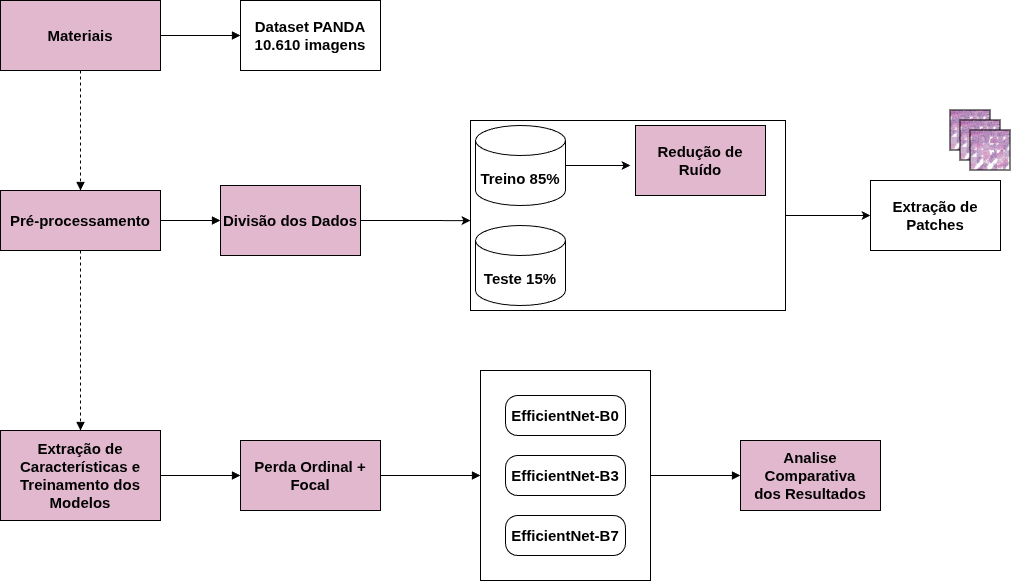
\includegraphics[width=0.9\linewidth]{images/method-semish.png}
    \caption{Proposed Method}
    \label{fig:method}
\end{figure}

\subsection{Materials}
\label{sub:data}

In this work, the PANDA dataset (\textit{Prostate Cancer Grade Assessment}) was used, comprising approximately 10,616 complete histopathological images (\textit{Whole Slide Images} - WSIs) from prostate biopsies \cite{ref-panda2020}. This dataset was released as part of the PANDA challenge on the Kaggle platform and has been widely used in research on the automatic classification of prostate cancer. The images in the dataset are annotated with the Gleason score and Gleason grade, providing clinical labels used for disease grading. In this study, only the public version of the dataset was used, without access to the private test set provided during the challenge.

The data were collected from two distinct medical centers, \textit{Radboud University Medical Center} and \textit{Karolinska Institute}, introducing institutional variability into the images. This variability is associated with differences in slide preparation protocols, scanning procedures, and annotation criteria, thereby making the experimental scenario more closely resemble real clinical practice.

In addition, the dataset contains noise inherent to the slide acquisition and annotation processes. Among these, visual artifacts include pen marks made by pathologists during slide analysis, as illustrated in Figure~\ref{fig:pen_mask}. There are also labeling-related sources of noise, such as disagreement among annotators in assigning histopathological grades. These factors increase the complexity of the automatic classification task and reflect challenges present in digital pathology practice.

\begin{figure}[htbp]
	\centering
	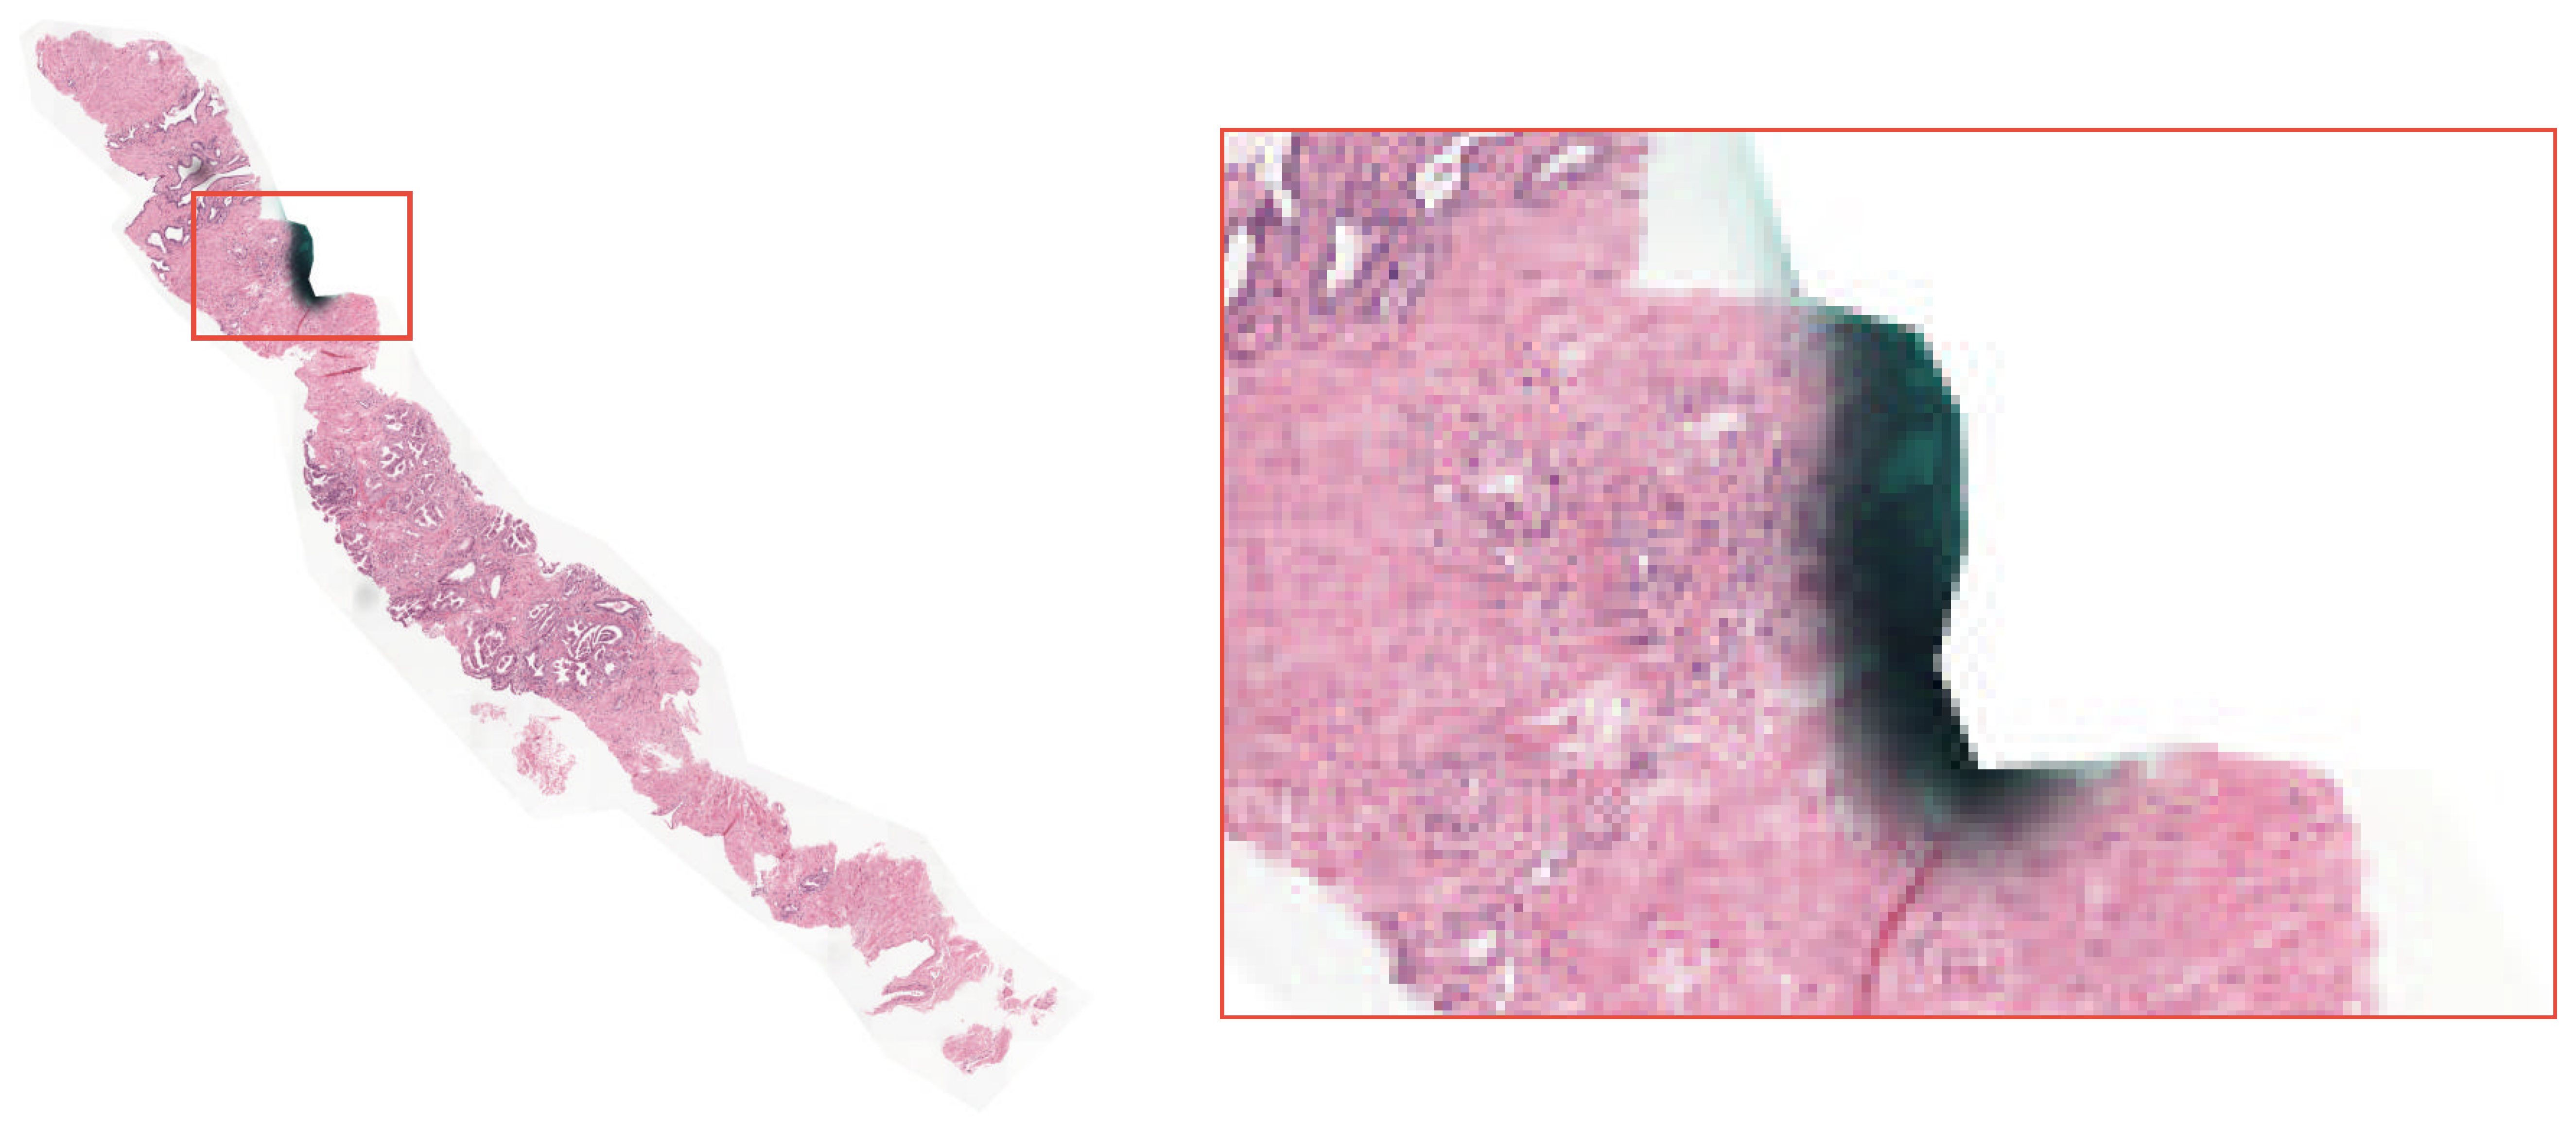
\includegraphics[width=0.8\linewidth]{images/zoom_region.png}
	\caption{Example of a visual artifact present in a WSI from the PANDA dataset. On the left, the complete slide is shown with the region of interest highlighted in red. On the right, an enlarged view of the selected region reveals a pen mark over the prostate tissue.}
	\label{fig:pen_mask}
\end{figure}

Another relevant aspect of the dataset is the unequal distribution of samples among the six ISUP grading classes (ISUP 0 to ISUP 5). It is noteworthy that ISUP grade 0 indicates the absence of malignant lesions. A higher concentration of samples is observed in ISUP classes 0 and 1, while the remaining classes are less represented. The complete distribution of samples is presented in Figure \ref{fig:distribuicao-isup}.

\begin{figure}[htb]
	\centering
	\includegraphics[width=1\textwidth,height=0.3\textheight]{"images/distribuição ISUP"}
	\caption{Distribution of samples in the PANDA dataset}
	\label{fig:distribuicao-isup}	
\end{figure}

\subsection{Preprocessing}

During the preprocessing phase, the data were initially divided into training and testing sets to ensure a clear separation between model fitting and evaluation. Subsequently, a noise reduction technique based on entropy was applied, followed by patch extraction based on the information density of each slide.

For the noise-reduction stage, four architectures based on the \textit{EfficientNet} backbone (B0, B1, B2, and B3) were used to compute Shannon entropy to quantify prediction uncertainty \cite{ali2023entropy}. The average entropy of the four models was calculated for each sample in the training set, and the top 10\% percentile was selected, forming a dataset of potentially noisy samples. From this subset, four scenarios were evaluated: retaining all data and removing 100\%, 50\%, and 20\% of the images identified as noisy. The best performance was obtained when removing 20\% of these images (180 samples), indicating that many samples, despite presenting high uncertainty, still contribute relevant information to the problem within the dataset context.

In the final stage of preprocessing, new images were generated from the PANDA WSIs through patch extraction, selecting regions containing relevant tissue. This approach was necessary because histological material occupies only part of the slide; without patch extraction, processing the original WSIs directly would incur high computational cost and analyze large non-tissue areas, as illustrated in Figure~\ref{fig:original-panda}.

\begin{figure}[htb]
\centering

\includegraphics[width=0.8\linewidth]{images/original.png}
\caption{Example image from the PANDA dataset}
\label{fig:original-panda}
\end{figure}

To determine the best extraction strategy, the reorganization of images into \textit{patches} was evaluated using configurations of 5×5 (25 \textit{patches}), 6×6 (36 \textit{patches}), and 7×7 (49 \textit{patches}). As illustrated in Figure~\ref{fig:tiles-original}, the 5×5 configuration presents a higher density of tissue and a smaller proportion of empty areas; however, the reduced number of fragments may lead to the loss of potentially relevant regions, impairing the representation of more subtle lesion patterns. On the other hand, the 7×7 configuration preserves greater spatial coverage of the slide but includes many regions without tissue and produces high-dimensional images (1792×1792), increasing memory requirements and processing time. Therefore, the intermediate configuration of 36 \textit{patches} was selected, as it preserves most of the tissue information while maintaining relatively reduced dimensionality (1536×1536), balancing quality, coverage, and computational efficiency.

\begin{figure}[H]
	\centering
	
\includegraphics[width=0.9\textwidth]{images/tiles-original.png}
	\caption{Illustration of patch extraction with different grid sizes: 5×5 (left), 6×6 (center), and 7×7 (right).}
	\label{fig:tiles-original}
\end{figure}

\subsection{Feature Extraction and Model Training}

This section presents the proposed approach for training the individual classifiers, including the definition of hyperparameters, regularization strategies, and the loss function. After preprocessing, model training and evaluation were initiated. EfficientNet-B0 was used as the base model for hyperparameter tuning. Once the configuration was defined, the experiments were extended to EfficientNet-B3 and B7, enabling comparisons across different complexity levels within the same family and analysis of the impact of increased representational capacity on performance and generalization.

Initially, \textit{Binary Cross-Entropy} (BCE) was adopted as the baseline loss function due to its widespread use in multilabel classification scenarios. From this initial configuration, exploratory experiments were conducted to assess training stability and the impact of hyperparameters on model generalization. Variations in the learning rate, the number of layers unfrozen during \textit{fine-tuning}, and regularization strategies through \textit{Dropout} were evaluated. To select the best hyperparameter combination, a systematic grid search was performed using the EfficientNet-B0 model. This search was conducted on a subset corresponding to 20\% of the training set, reserved for internal validation, enabling identification of the best-performing configuration before the final training stage.

Despite evaluating these configurations during training, performance stagnation was observed, which could be attributed not only to the choice of hyperparameters but also to the formulation of the loss function. Given that prostate cancer grading is ordinal, with errors between adjacent classes less severe than those between more distant classes, the problem was reformulated as an ordinal regression task.

In this formulation, ISUP grade prediction is not treated as a multiclass problem with independent categories but rather as a sequence of cumulative binary classifications. For an ISUP grade $k \in \{0,\dots,5\}$, the label is encoded as a cumulative binary vector in which the first $k$ elements assume value 1 and the remaining elements 0; for example, grade 3 is represented as $[1,1,1,0,0]$. The ordinal loss is then applied independently to each threshold in the vector, yielding a total error that corresponds to the sum of cumulative discrepancies. This modeling imposes a penalty proportional to the distance between classes, such that more distant errors incur greater cost, preserving the hierarchical structure of the problem.

To mitigate class imbalance (Section \ref{sub:data}), the ordinal loss was combined with \textit{Focal Loss} \cite{lin2017focal, DINA2023100699, CHEN2026235}. This function modulates cross-entropy to reduce the influence of highly confident predictions, prioritizing samples with greater diagnostic uncertainty. In this study, the focusing factor $\gamma = 2.0$ was used to attenuate the contribution of easy examples, and the weight $\alpha = 0.25$ was used to balance the relative importance among classes. This strategy directs optimization toward more complex and underrepresented cases, which are essential for precise discrimination between ISUP grades.

\subsection{Evaluation Metrics}

The metrics used were \textbf{accuracy} and \textbf{$\kappa_{\text{quad}}$} (Quadratic Weighted Kappa). Accuracy measures the proportion of correct predictions relative to the total number of evaluated instances \cite{baldi2000assessing}. The $\kappa_{\text{quad}}$ metric quantifies the degree of agreement between predicted and true classes while incorporating penalties proportional to the magnitude of the error, making it particularly suitable for ordinal problems \cite{ref-cohen1968}.

The variability of the metrics and their respective confidence intervals were estimated using nonparametric bootstrap \cite{efron1979bootstrap}. Based on predictions from the test set, 1,000 resamples with replacement were generated while preserving the original dataset's size. For each iteration, the performance indicators were recalculated, enabling estimation of the mean, standard deviation, and 90\% confidence interval (CI) based on the 5\% and 95\% percentiles. This approach provides a robust uncertainty estimate without requiring parametric assumptions about the data distribution.